\documentclass[12pt]{article}
\usepackage{geometry}

%\usepackage[margin=0.2in]{geometry}                
\geometry{letterpaper}                  
\usepackage{graphicx}
\usepackage{tipa}
\usepackage{upgreek}
\usepackage{amsmath, amssymb, amsthm}
\newtheorem{theorem}{Theorem}
\newtheorem{corollary}{Corollary}
\newtheorem{proposition}{Proposition}
\newtheorem{lemma}{Lemma}
\newtheorem{definition}{Definition}
\newtheorem{remark}{Remark}
\newtheorem{notation}{Notation}
\newcommand{\N}{\mathcal{N}}
\newcommand{\Bern}{\textrm{Bern}}
\newcommand{\Bin}{\textrm{Bin}}
\newcommand{\Beta}{\textrm{Beta}}
\newcommand{\Gam}{\textrm{Gamma}}
\newcommand{\Expo}{\textrm{Expo}}
\newcommand{\Pois}{\textrm{Pois}}
\newcommand{\Geom}{\textrm{Geom}}
\begin{document}

\begin{center} \textbf{Programming Assignment 3} \end{center}
 \vspace{-8mm} 
\begin{center} \textbf{Perry Green \& Julia Winn} \end{center}

\noindent \textbf{Dynamic Programming}
\medskip

\noindent Given a set of $n$ numbers A and the knowledge that these numbers sum up to $b$, there are several ways we can solve the partition problem.
\medskip

\noindent \textbf{Naive Solution}
\medskip

\noindent Say that the set of numbers is stored in array A of length $n$. For the naive solution we create an array B of dimensions $(n+1) \times (b+1)$.  In general, non-Null entries in row $i$ represent possible sums that can be achieved using some or all of the first $i$ numbers in the set. So, initialize the first cell B[0][0] to be a pointer to itself and fill the rest of the row with Null pointers, since with the empty-set you can only get a sum of 0.
\medskip

\noindent The remainder of the matrix is filled out as dictated by the recurrence: 
$$B[i][j] = B[i-1][j] \textbf{ } || \textbf{ } B[i-1][j-A[i-1]]$$

\noindent If both of the entries on the right hand side are Null, set B[i][j] to Null. Otherwise, set B[i][j] to a pointer to one of the non-Null cells (if both are non-Null, choose one arbitrarily). This represents the idea that you can get a number $j$ using the first $i$ members of $A$ EITHER if you can get the number $j$ with the first $i-1$ members, OR if you can get the number $j-A[i-1]$ with the first $i-1$, such that adding in the $i$th number raises the sum to $j$.
\medskip

\noindent Our algorithm is complete when we have arrived at the index B[$(n+1),(b+1)]$.  At this point, the bottom row are the possible values a subset of the values can take. We traverse the bottom row and find the non-Null cell closest to $b/2$, which represents one of the sets in the partition which minimizes the residue.  Call this cell B$[n][j_0]$. $2*(b/2-j_0)$ is the difference between these two sets, and so is the residue. To find the numbers which actually make up this set, follow the pointers backwards. If B$[n][j_0]$ points to B$[n-1][j_1]$, then $j_0-j_1$ must be in the set. Repeat this process until you reach B[0][0].
\medskip

\noindent One big disadvantage of this approach is that it takes up much more space than it needs too. As we explain below, it is possible to reuse a single row to use $O(b)$ space instead of $O(nb)$ space. But, this other strategy doesn't lend itself to a nice recurrence equation like we have for this one, so we chose to include this worse solution as well.
\medskip

\noindent \textbf{Better Solution}
\medskip

\noindent We begin with a one dimensional array of length $b/2 + 1$, one can round up or down should this not be an even number, it should not affect the solution because if our $b$  In this instance we will round down. The index B[i] is true only if there exists a subset of numbers that sum to $i$.  Because we know if we can find one combination of numbers that sums to half of the total sum the other half of the numbers must also sum to half the total sum.  Initialize this array to have every variable be Null except B[0], which points to itself, because we can reach the sum zero using the empty set.
\medskip

\noindent Now beginning with A[0], set B[A[0]] to point to B[0].  Continuing on for all other values in A, or, for i in range 1 to len(A):
\\ \indent Set B[A[i]] to point to B[0]
\\ \indent Starting at B[b/2+1] and going backwards down the array until we reach B[0]:
\\ \indent \indent For all indices of B that are pointing to something: (call each instance B[j])
\\ \indent \indent If A[i] + a non null index of B[j] $< b/2$ then set B[B[j] + A[i]] to point to B[j] 
\\ \indent If looking for an exact solution of residue 0, then if at any point B[b/2+1] is no longer Null, return true and/or the combination of numbers. (see below) If you run out of numbers in your set and this has not happened, return false.
\\ \indent If looking for the optimal solution, then find the square closest to the final index, and return the combination of numbers leading to this square (see below).
\medskip

\noindent Starting with index b/2 +1, or your highest index of choice (minimum residue) go to the index this one is pointing to, subtract this index from b/2+2 (or your highest index), and add the difference to the list of numbers in this half of the partition.  Once a number points to itself we have reached the first index, so return the value of the previous index, which would also be itself minus 0, which is equivalent to the value of the previous index.
\bigskip

\noindent 
\bigskip

\noindent \textbf{Karmarkar-Karp in $O(n\log n)$ time}
\medskip

\noindent You have $n$ numbers, small enough that so that arithmetic operations take one step. Start by constructing a max-heap with the $n$ numbers, which takes $O(n)$ time. Then, $n-1$ times: pop off 2 numbers, find their difference, and then insert the difference back into the heap. Both inserting and popping are $O(log(n))$, so the 3 heap operations and 1 arithmetic operation are $O(log(n))$. Since you repeat this process $n-1$ times, in total it is $O(nlog(n))$. Each time you pop/insert, you reduce the size of the heap by $1$. So, in the end, there is one number left. Return the one remaining number.

Correctness follows by the structure of the heap. Since the head of the heap is always the largest number, each iteration you are replacing the two largest elements in the set with their difference. When you get down to one element, you return it, just like in Karmarkar-Karp.

\bigskip

\begin{center} \textbf{Graphs} \end{center}

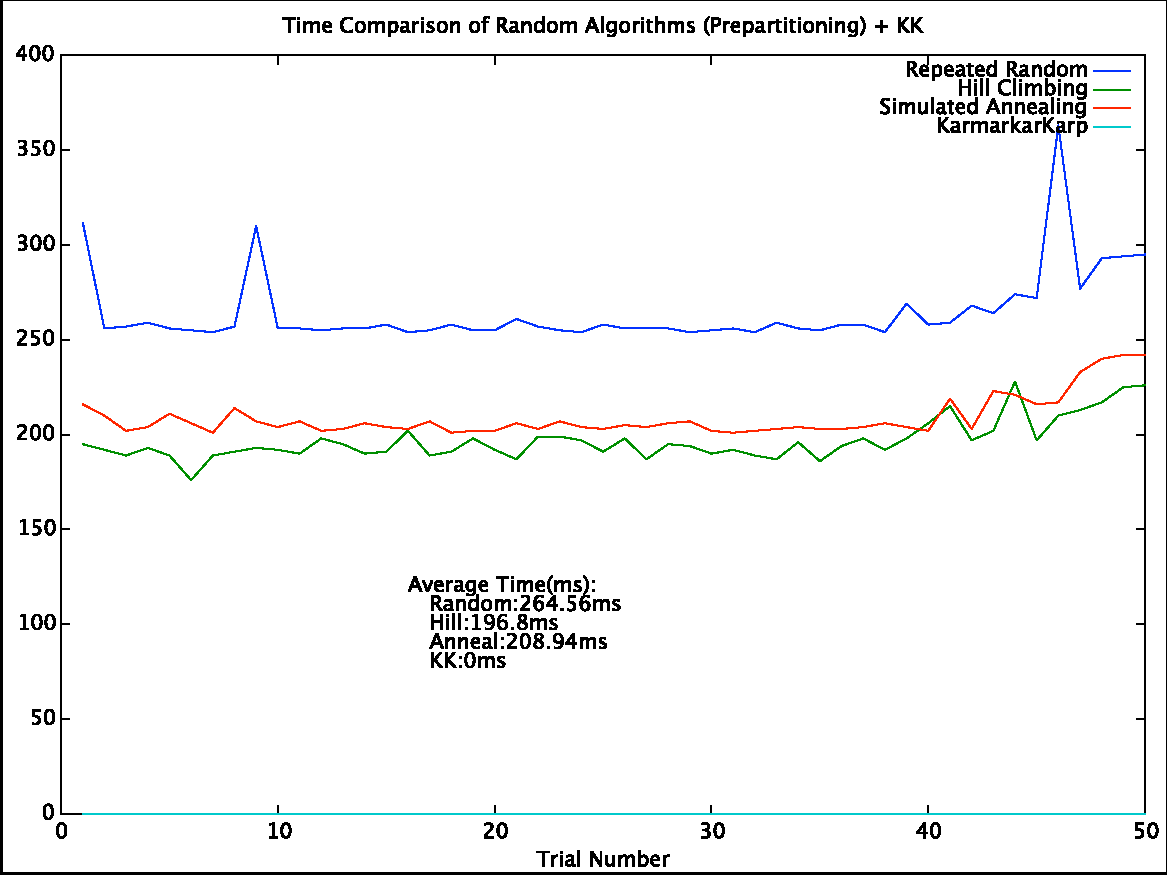
\includegraphics[scale=0.8]{false_time.pdf}
\noindent In the middle of this trial we think something odd happened on my computer, and the increase we see at the end is not a reflection of our algorithms, but of hardware activity.  The initial drop we wee with repeated random is similar to what we see in the next graph- to be explained then.
\\
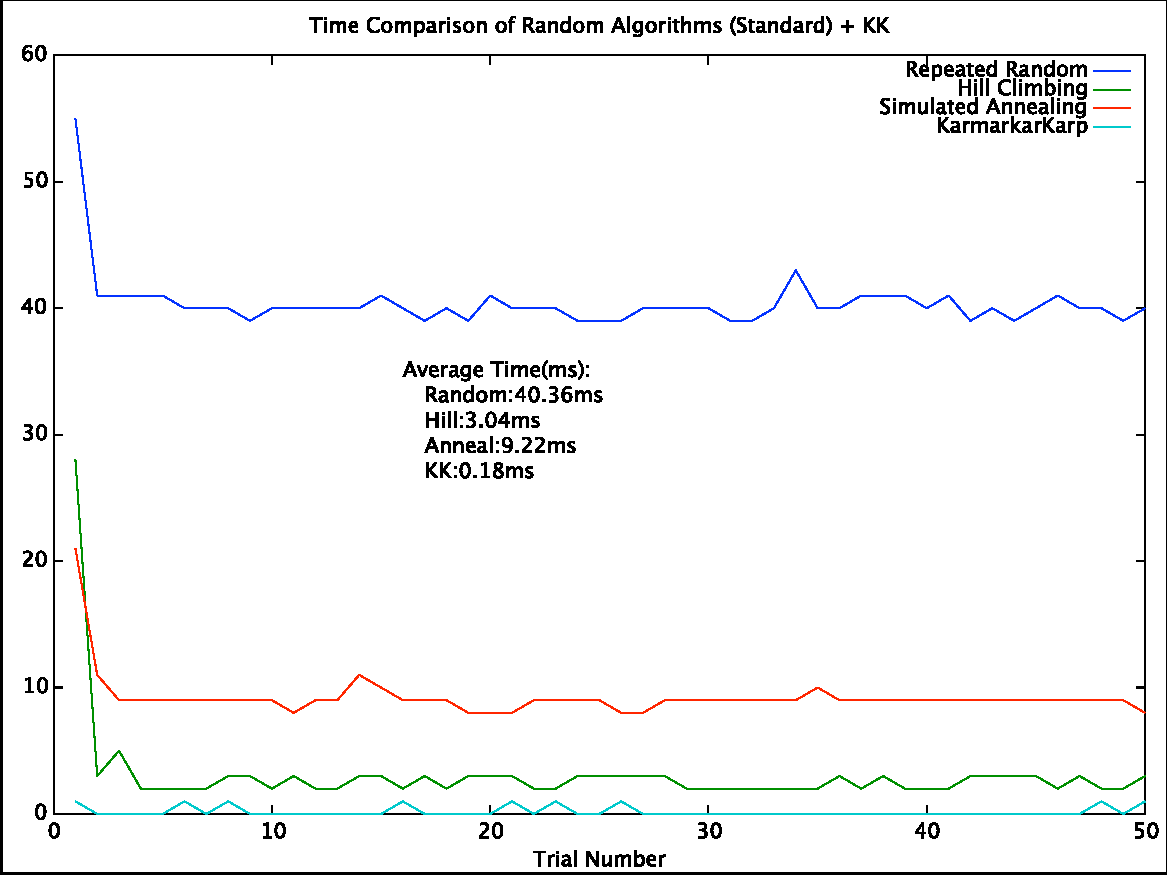
\includegraphics[scale=0.8]{true_time.pdf}
\noindent We see a sharp decrease in time from the first trial(s) to the second or third trial, similarly to what we viewed for repeated random in the graph above.  We attribute this to the Java virtual machine's optimization that it perfects after an iteration.
\\
 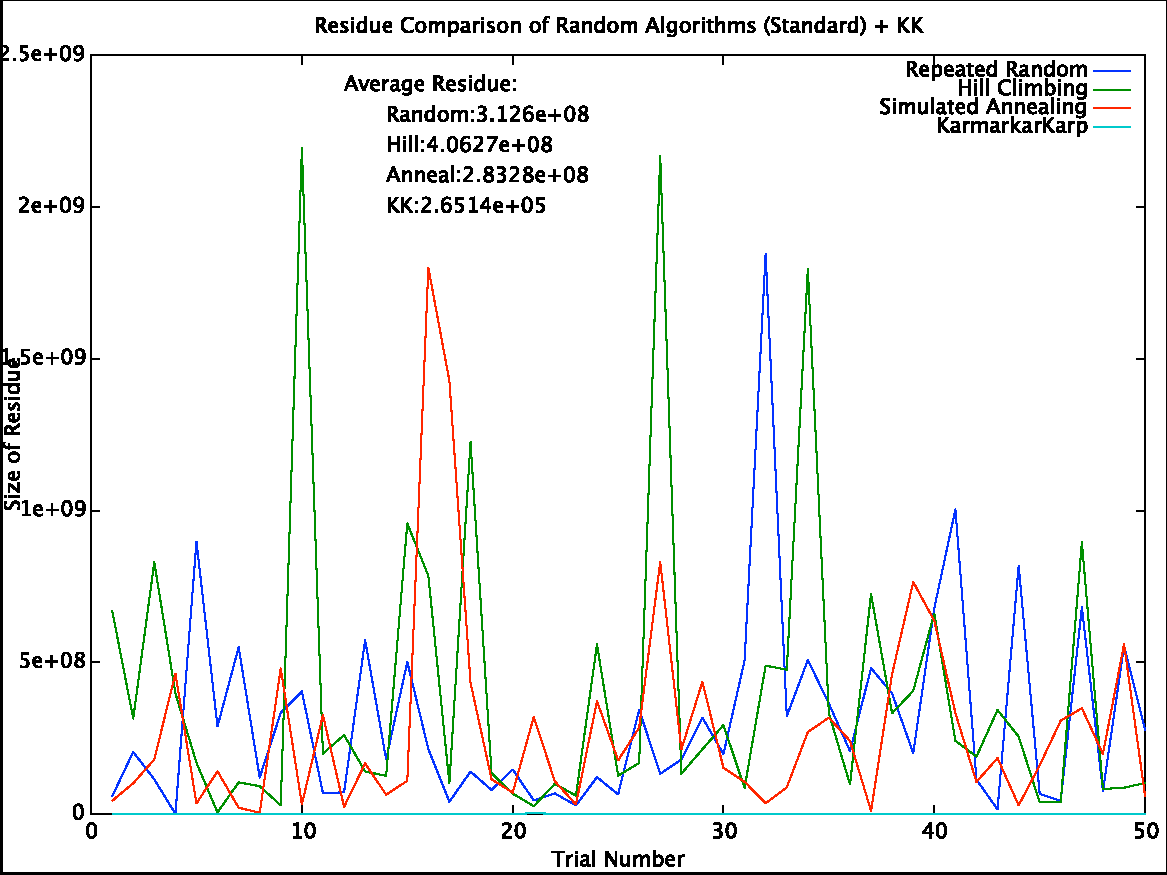
\includegraphics[scale=0.8]{true_values.pdf} 
 \noindent In this instance Karmarkar-Karp is the clear winner, it's line is barely visible in this graph where most residues are in the billions.
\\
 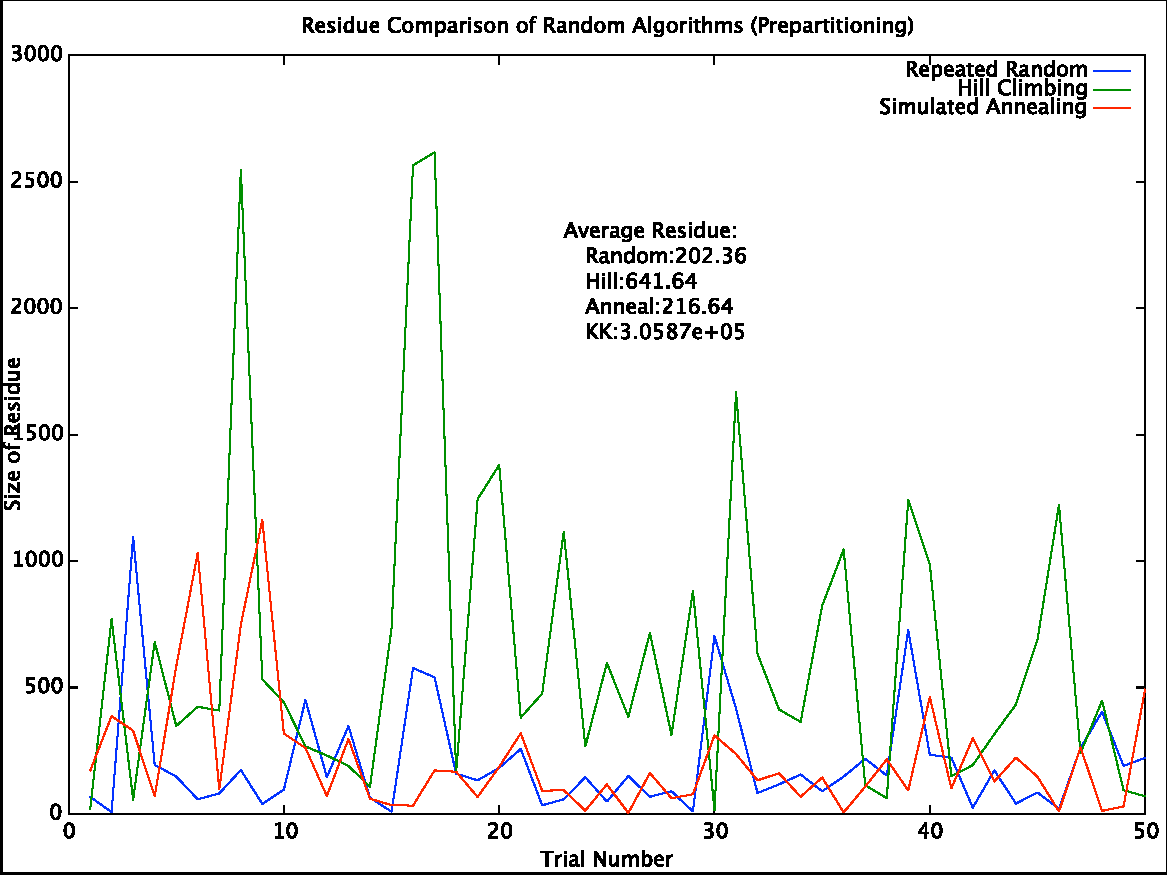
\includegraphics[scale=0.8]{false_values.pdf} 
 \\
 \noindent We ran KK again (above) but it was so much worse than the other algorithms that we had to not depict it on the graph so that we could see the differences between the first 3 random methods.  
 \medskip
 
 \noindent \textbf{Graph Comparisons}
 \medskip
 
 \noindent Looking at the differences between the pre-partitioned implementation and the standard implementation for time you can see that pre-partitioning is more costly with regards to time, the average values being $\approx$ 5 times higher than the highest time for standard algorithms (40- repeated random to 200-hill climbing and simulated annealing), and 20 to 25 times higher than the lower averages (3- standard hill climbing and 9- standard annealing compared to $\approx$ 200 for their pre-partitioned counterpoints).  Karmarkar-Karp is consistently near 0 when it comes to time cost for both pre-partitioned and standard implementations.
 \bigskip
 
 \noindent However when considering the residue, a reflection of the correctness when comparing the results of different algorithms running identical sets of numbers, we see that with pre-partitioning the residues for the other algorithms plummet dramatically and where Karmarkar-Karp was previously the best by several orders of magnitude, this is no longer the case, where the random algorithms all average below 1000.  This is expected, because with pre-partitioning Karmarkar-Karp is being called repeatedly by the random algorithms, and as a result, their accuracy is very high.
 \medskip
 
 \noindent \textbf{Karmarkar-Karp with Randomized Algorithms}
\medskip
 
 \noindent \emph{Karmarkar-Karp as a starting point}: All of our random algorithms start by generating a random solution. Instead, we might purposefully select an appropriate starting solution, such as the result of running Karmarkar-Karp. This would be done by running Karmarkar-Karp, and passing that as an argument to the random algorithms, which would then use that as the initial `best' solutions, instead of a randomly generated one.

For the repeated-random algorithm, this has the effect of setting a lower-bound: no matter `unlucky' you are in generating random solutions, you won't end up returning a solution worse than Karmarkar-Karp. This might be useful if, for some reason, you had to run very few iterations, or possibly you can't be sure how many iterations will be run. For example, you might run repeated-random until some event occurs, which could be a very short period of time. However, as soon as a solution better than Karmarkar-Karp's is randomly generated, the initial solution is no longer relevant. So, when there is time to run many iterations, starting with Karmarkar-Karp is likely to be an irrelevant waste of time. In fact, given the results about the speed of the algorithms and their relative efficacy in the preceding plots, this latter case is the most likely, and it isn't worth starting with the Karmarkar-Karp solution when doing the repeated-random algorithm.

For hill-climbing and simulated-annealing, Karmarkar-Karp also serves as a lower bound. But, more importantly, it dictates the region in the solution space which you search around. Instead of searching around a random part of the solution space, you search near a solution which is at least ok.  When doing very few iterations, this could be very good, since it bypasses whatever iterations are necessary to move from a terrible (randomly generated) solution to a reasonable one. Running hill-climbing and simulated-annealing from this starting point will search around that area, and presumably find a local minimum. Since Karmarkar-Karp is likely to be better than a random solution, it will take fewer iterations to find/get close to a local minimum. But, that won't necessarily improve the algorithm, since it doesn't take that much time/that many iterations (at least using the prepartition solution) to get close to a local minimum. The relevant question is which of the local minima found, starting either randomly or using Karmarkar-Karp, is likely to be better. We can't find any reason to believe that Karmarkar-Karp should be significantly closer to the \emph{universal} minimum than a random solution. So, given a number of iterations of the same order used in this assignment, it is unlikely that Karmarkar-Karp would meaningfully affect the results of the random algorithms.

%\begin{itemize}  \itemsep1pt \parskip0pt \parsep0pt
%\item 
%\end{itemize}




\end{document}